\documentclass[10pt,a4paper,twocolumn,twoside]{article}
\usepackage[utf8]{inputenc}
\usepackage[catalan]{babel}
\usepackage{multicol}
\usepackage{graphicx}
\usepackage{fancyhdr}
\usepackage{times}
\usepackage{titlesec}
\usepackage{multirow}
\usepackage{lettrine}
\usepackage{cite}
\usepackage{array}
\usepackage[table,xcdraw]{xcolor}
\usepackage{subfig}
\usepackage{listings}
\usepackage[top=2cm, bottom=1.5cm, left=2cm, right=2cm]{geometry}
\usepackage[figurename=Fig.,tablename=TAULA]{caption}
\usepackage{stackengine}
\captionsetup[table]{textfont=sc}

\usepackage{xcolor}
\setcounter{secnumdepth}{4}
\titleformat{\paragraph}
{\normalfont\normalsize\bfseries}{\theparagraph}{1em}{}
\titlespacing*{\paragraph}{0pt}{3.25ex plus 1ex minus .2ex}{1.5ex plus .2ex}

\definecolor{codegreen}{rgb}{0,0.6,0}
\definecolor{codegray}{rgb}{0.5,0.5,0.5}
\definecolor{codepurple}{rgb}{0.58,0,0.82}
\definecolor{backcolour}{rgb}{0.95,0.95,0.92}

\lstdefinestyle{mystyle}{
    backgroundcolor=\color{backcolour},   
    commentstyle=\color{codegreen},
    keywordstyle=\color{magenta},
    numberstyle=\tiny\color{codegray},
    stringstyle=\color{codepurple},
    basicstyle=\ttfamily\footnotesize,
    breakatwhitespace=false,         
    breaklines=true,                 
    captionpos=b,                    
    keepspaces=true,                 
    numbers=left,                    
    numbersep=5pt,                  
    showspaces=false,                
    showstringspaces=false,
    showtabs=false,                  
    tabsize=2
}

\lstset{style=mystyle}


\author{\LARGE\sffamily Ricard López Olivares}
\title{\Huge{\sffamily Robot Industrial Stäubli TX60 com a classificador de residus}}
\date{}

\newcommand\blfootnote[1]{%
  \begingroup
  \renewcommand\thefootnote{}\footnote{#1}%
  \addtocounter{footnote}{-1}%
  \endgroup
}

%
%\large\bfseries\sffamily
\titleformat{\section}
{\large\sffamily\scshape\bfseries}
{\textbf{\thesection}}{1em}{}

\begin{document}

\fancyhead[LO]{\scriptsize AUTOR: Ricard López Olivares}
\fancyhead[RO]{\thepage}
\fancyhead[LE]{\thepage}
\fancyhead[RE]{\scriptsize EE/UAB TFG INFORMÀTICA:Robot Industrial Säubli TX60 com a classificador de residus}

\fancyfoot[CO,CE]{}

\fancypagestyle{primerapagina}
{
   \fancyhf{}
   \fancyhead[L]{\scriptsize TFG EN ENGINYERIA INFORMÀTICA, ESCOLA D'ENGINYERIA (EE), UNIVERSITAT AUTÒNOMA DE BARCELONA (UAB)}
   \fancyfoot[C]{\scriptsize Juny de 2023, Escola d'Enginyeria (UAB)}
}

%\lhead{\thepage}
%\chead{}
%\rhead{\tiny EE/UAB TFG INFORMÀTICA: TÍTOL (ABREUJAT SI ÉS MOLT LLARG)}
%\lhead{ EE/UAB \thepage}
%\lfoot{}
%\cfoot{\tiny{Mes 2023, Escola d'Enginyeria (UAB)}}
%\rfoot{}
\renewcommand{\headrulewidth}{0pt}
\renewcommand{\footrulewidth}{0pt}
\pagestyle{fancy}

%\thispagestyle{myheadings}
\twocolumn[\begin{@twocolumnfalse}

%\vspace*{-1cm}{\scriptsize TFG EN ENGINYERIA INFORMÀTICA, ESCOLA D'ENGINYERIA (EE), UNIVERSITAT AUTÒNOMA DE BARCELONA (UAB)}

\maketitle

\thispagestyle{primerapagina}
%\twocolumn[\begin{@twocolumnfalse}
%\maketitle
%\begin{abstract}
\begin{center}
\parbox{0.915\textwidth}
{\sffamily
\textbf{Resum--}
La robòtica ha transformat la nostra vida quotidiana de diverses maneres. Des de robots domèstics que realitzen tasques de la llar fins a sistemes automatitzats a indústries i hospitals, els robots estan cada vegada més presents. Han millorat l'eficiència i la precisió en la fabricació i l'atenció mèdica, i han facilitat la realització de tasques repetitives i perilloses. A més, els avenços en la intel·ligència artificial han permès el desenvolupament de robots autònoms i col·laboratius, que interactuen amb els humans de manera més natural. \\
En aquest treball s'ha utilitzat un robot Stäubli Tx60 i s'ha incorporat la visió per computador, aquest robot té dues comunicacions una amb un PLC, que li diu la velocitat de la cinta i si hi ha objecte, en cas que hi hagi un objecte enviarà un senyal al robot i aquest a l'ordinador per posar en marxa la visió per computador i classificar l'objecte, un cop classificat s'envia al robot el resultat i mou l'objecte a la seva zona.
\\
\\
\textbf{Paraules clau-- } Robot, Tx60, Stäubli, antropomòrfic, intel·ligència artificial, classificador, xarxa neuronal, residus, industrial, DenseNet-121, Val3, Python, Sockets.
\\
%\end{abstract}
%\bigskip
%\begin{abstract}
\bigskip
\\
\textbf{Abstract--} Robotics has transformed our daily lives in various ways. From domestic robots that perform household tasks to automated systems in industries and hospitals, robots are becoming increasingly present. They have improved efficiency and accuracy in manufacturing and healthcare, and have facilitated the execution of repetitive and dangerous tasks. Furthermore, advancements in artificial intelligence have enabled the development of autonomous and collaborative robots that interact with humans in a more natural way. \\
In this project, a Stäubli Tx60 robot was used, incorporating computer vision. This robot has two communications: one with a PLC, which informs it of the conveyor belt's speed and detects the presence of an object. If an object is detected, a signal is sent to the robot and the computer activates computer vision to classify the object. Once classified, the result is sent back to the robot, which then moves the object to its designated area.
\\
\\
\textbf{Keywords-- }  Robot, Tx60, Stäubli, anthropomorphic, artificial intelligence, classifier, neural network, waste, industrial, DenseNet-121, Val3, Python, Sockets.
\\
}

\bigskip

{\vrule depth 0pt height 0.5pt width 4cm\hspace{7.5pt}%
\raisebox{-3.5pt}{\fontfamily{pzd}\fontencoding{U}\fontseries{m}\fontshape{n}\fontsize{11}{12}\selectfont\char70}%
\hspace{7.5pt}\vrule depth 0pt height 0.5pt width 4cm\relax}

\end{center}

\bigskip
%\end{abstract}
\end{@twocolumnfalse}]

\blfootnote{$\bullet$ E-mail de contacte: ricardlopezolivares@gmail.com}
\blfootnote{$\bullet$ Menció realitzada: Computació}
\blfootnote{$\bullet$ Treball tutoritzat per: Carlos García Calvo (Departament de Ciències de la Computació)}
\blfootnote{$\bullet$ Curs 2022/23}

\section{Introducció}

\lettrine[lines=3]{E}{n} l'era de la Indústria 4.0, la necessitat de solucions innovadores per abordar els reptes del reciclatge i la sostenibilitat es fa cada vegada més urgent. En aquest emocionant projecte, es busca crear un canvi significatiu en combinar la tecnologia de xarxes neuronals amb un robot de reciclatge d'avantguarda. L'objectiu principal és revolucionar la forma en què es gestionen els residus i fomentar una economia circular més eficient. Aquest robot autònom està dissenyat per identificar i classificar de manera precisa i eficient els materials reciclables, com ara plàstics, vidres,  metalls, paper, cartró, etc, en corrents de deixalles.
\\

La clau d'aquest projecte rau en la implementació de xarxes neuronals, que permeten al robot aprendre i adaptar-se a diferents tipus de materials a mesura que es troben en el procés de reciclatge. La integració en el marc de la Indústria 4.0 proporciona un avantatge addicional en permetre el monitoratge en temps real i l'anàlisi de dades, cosa que optimitza encara més el procés de reciclatge i permet identificar i solucionar problemes de manera eficient. En millorar l'eficiència i la precisió en la classificació dels materials reciclables, aquest enfocament innovador té com a objectiu maximitzar la recuperació de recursos i reduir la quantitat de residus que acaben en abocadors. En última instància, aquest projecte representa un pas endavant cap a un futur més conscient i responsable pel que fa a la gestió dels recursos naturals i la cura del medi ambient.
\\

El projecte el podem dividir en tres grans parts, aquestes són:

\begin{itemize}
  \item Robòtica: En aquest apartat trobaríem el robot utilitzat, Säubli TX60 \cite{TX60}, amb la seva controladora, CS8C\cite{CS8C}, una pinça pneumàtica i el simulador,Stäubli robotics suite 2022\cite{SRS} .
  \item Sistema de visió: Aquest apartat és el que intenta que el robot pugui classificar els objectes obtinguts. L'apartat consta de la xarxa neural empleada, DenseNet-121\cite{DenseNet} i càmera d'un telèfon mòbil, Iphone XR\cite{IphoneXR}.
  \item Sistemes industrials: En aquest apartat trobem una cinta per transportar els objectes d'un punt a un altre, amb un motor trifàsic, un PLC 1200 AC, un variador de velocitat de la marca Omron MX2-A2002 i un sensor d'objectes de la marca Omron E3FA-DP12.
\end{itemize}

\section{Objectius}

En el projecte tenim dos objectius principals, el primer és crear una simulació de tot el treball final, aquesta s'ha de semblar el més possible a la realitat, el segon és la creació d'aquest projecte en un àmbit real.
\\

Com aquests dos objectius són massa general/globals, els que s'ha fet és dividir aquests en objectius més petits, aquest son: realització d'identificació d'objectes, buscar un programa simulador que ens permeti recrear el món real, crear l'escenari de la simulació, utilització d'una pinça pneumàtica, familiaritzar-se amb el llenguatge i codificació d'un robot industrial, connexió entre les diferents parts i enviar dades entre elles.
\\
\hfill \break
(Consultí l’annex A.1 per veure més informació sobre els objectius.)

\section{Planificació}

En aquest projecte s'ha decidit fer una divisió en tasques els objectius, ja que no tots els objectius formen part del projecte final, sinó que són passes necessàries per poder arribar al producte final. D'aquesta manera el projecte ens proporciona una flexibilitat de fer les tasques sense que depengui una amb un altre i paral·lelitzar unes amb un altre, és a dir, fer més d'una tasca al mateix temps.
\\

Un cop tenim totes les tasques vaig plantejar utilitzar una metodologia àgil o agile, la qual s'adapti a les necessitats del projecte en aquest punt, la metodologia aplicada s'anomena Kanban\cite{Kanban}, aquesta consisteix a tenir un taulell amb diferents columnes, i totes les tasques se situen a la primera columna i aquestes només es mouran de columna segons el desenvolupament de la tasca, un exemple del taulell es pot veure a la Figura 1.

\begin{figure}[h]
\centering
	\includegraphics[width=0.5\textwidth]{img/kanban}
	\caption{Exemple de taulell kanban}
	\label{fig-taulell canban}
\end{figure}

\hfill \break
(Consultí l’annex A.2 per veure més informació sobre la planificació.)

\section{Especificacions i tecnologies empleades }

Per realitzar aquest projecte s'han necesitat diversos components esencials, aquest son:

\begin{itemize}
  \item \textbf{Robot Stäubli TX60}: S'ha decidit aquest robot per les seves característiques i la seva àrea de treball, aquesta última es refereix a tots els punts on el robot pot arribar sense cap mena de problemes, la seva forma és un torus, ja que d'aquesta forma el robot evita la col·lisió amb si mateix. Les següents figures mostren l'àrea de treball.

\hfill \break
(Consultí l’annex A.2.1 per veure més informació sobre les caracteristíques del TX60.)
\begin{figure}[h]
 \centering
  \subfloat[Perfil]{
   \label{f:perfil}
    \includegraphics[width=0.2\textwidth]{img/tx60.png}}
  \subfloat[Alçada]{
   \label{f:alçada}
    \includegraphics[width=0.2\textwidth]{img/tx60altura.png}}
 \caption{Àrees de treball TX60}
 \label{f:tx60}
\end{figure}

  \item\textbf{Controlador CS8C}: Sempre que utilitzem un robot industrial es necessita una controladora, aquesta s'encarrega d'enviar-li al robot les instruccions que ha de fer, la controladora sempre va amb un comandament manal per controlar el robot manualment.

\begin{figure}[h]
 \centering
  \subfloat[CS8C]{
   \label{f:CS8C}
    \includegraphics[width=0.265\textwidth]{img/CS8C.jpg}}
  \subfloat[Comandament]{
   \label{f:comandament}
    \includegraphics[width=0.15\textwidth]{img/comandament.jpg}}
 \caption{Controladora CS8C i comandament}
 \label{f:tx60}
\end{figure}
\hfill \break
\hfill \break
\\
\\
\\
\\
\\
  \item\textbf{Simulador Stäubli robotic suite}: Aquest software ens permet treballar únicament amb els robots de l'empresa Stäubli, però d'una manera fàcil, amigable i el més real possible, ja que es poden simular tots els components del robot i entrades del controlador per fer una simulació el més pròxim a la realitat possible, també ens permet programar des de la posada en marxa del robot fins a l'aturada, optimització del rendiment, detecció i previsió de col·lisions, calibració, entre molts altres avantatges. Aquest simulador utilitza el mateix llenguatge que el robot real anomenat, VAL 3\cite{val3}.

  \item\textbf{PLC 1200 AC i variador de velocitat Omron Mx2-A2002}: Un PLC és un dispositiu electrònic utilitzat en l'automatització industrial per a controlar i supervisar altres sistemes i processos a temps real. Aquest tenen uns seguits d'entrades i sortides, poden ser digitals o analògiques, que es poden configurar per rebre informació de sensors o dispositius externs. Hi ha diferents estils de llenguatges per a un PLC, en aquest cas he fet servir un llenguatge de programació en blocs funcionals amb el programa  TIA PORTAL[17].
\\

Per altra banda, tenim el variador de velocitat Omron Mx2-AC2002, aquest dispositiu ens permet modificar la velocitat d'un motor trifàsic que dona un rang de potència d'entre 0.4 KW a 15 KW.

\begin{figure}[h]
 \centering
    \includegraphics[width=0.35\textwidth]{img/PLC.jpg}
    \caption{PLC 1200 AC i variador de velocitat Omron Mx2-AC2002}
\end{figure}

 \item\textbf{Sensor d'objectes Omron E3FA-DP12}: És un dispositiu dissenyat per detectar la presència o absència d'objectes en aplicacions industrials. Utilitzant la tecnologia de detecció per reflexió difusa, aquest sensor és capaç de detectar objectes sòlids en una varietat d'entorns i condicions.

  \item\textbf{Xarxa Neural}: La xarxa neural és qui dóna la intel·ligència de classificar en aquest projecte, aquesta s'ha implementat mitjançant TensorFlow\cite{TensorFlow}. TensorFlow és una biblioteca de codi obert utilitzada per l'aprenentatge automàtic d'intel·ligència artificial. Proporciona un conjunt d'eines i funcions per construir i entrenar models de xarxes neuronals. Tensorflow és molt emprat en aplicacions de processament d'imatges, llenguatge natural, etc.

  \item\textbf{Socket i IvCAM}:Les connexions entre dispositius són essencials per poder transmetre dades entre aquests, en aquest projecte es poden veure 2 tipus de connexions:
   \begin{itemize}
      \item \textbf{Sockets}\cite{sockets}: Aquest tipus de connexió ens permet la comunicació entre processos/dispositius a través d'una xarxa, la connexió funciona amb una estructura client - servidor. La connexió empleada en el projecte són sockets TCP.

      \item \textbf{IvCAM}\cite{IvCAM}: Aquesta connexió ens permet transferir dades d'imatges en temps reals. Per ajudar amb aquesta tecnologia hi ha un programa amb el mateix nom el qual ens ajuda a connectar la càmera d'un dispositiu a un altre, aquests dispositius han d'estar en la mateixa xarxa.
   \end{itemize}

  \item \textbf{GitHub}\cite{GitHub}: A l'hora de fer un projecte, ajuda molt tenir un control sobre les versions, veure un historial de canvis i poder anar enrere sempre que en necessiti, per tant, GitHub ha sigut una eina bastant útil en el desenvolupament del projecte.
\end{itemize}

\section{Desenvolupament}

En aquesta secció s'explica amb més deteniment, com s'ha desenvolupat el projecte durant aquest temps i per quines fases ha passat el mateix. 
\\

També cal mencionar que algunes d'aquestes fases es dividiran en més subseccions, pel fet que el projecte té 2 objectius finals (una simulació i un producte físic) o perquè  és una secció bastant global.

\subsection{Inici i planificació}

En primer lloc, s'ha determinat l'enfoc del projecte i en l'àmbit en el qual està enfocat amb la proposta. Tenint en compte els elements que tenim a l'abast.
\\

Un cop decidit l'àmbit en el qual es desenvolupa el projecte vaig fer una identificació d'objectiu, tal com s'explica en la secció 2 d'aquest document. A continuació, totes les tasques que han sortit es posen en un taulell i es va seguint la metodologia kanban, en cas que surti alguna tasca a posteriori o es vulgui eliminar, no afectaría, al ser una metodologia àgil es poden afegir o eliminar tasques sense cap problemes, però sempre seguint els principis de kanban.
\\
\\
\\
\\

Un cop tinc la vista global amb la majoria de les tasques que surten en un inici, vaig buscar eines i tecnologies que puguin resoldre les tasques a fer, sempre amb un mínim de dues tecnologies, d'aquesta forma si la primera no dona resultats tinc la segona i així evito fer tantes recerques per buscar de noves.
\subsection{Primeres passes}

En l'apartat anterior he mencionat que vaig buscar informació sobre les tasques per poder-les realitzar, i em vaig trobar que en algunes parts importants del projecte no es podia aplicar coneixements adquirits anteriorment, una situació d'aquest estil és amb el robot TX60 que funciona amb un llenguatge anomenat Val 3, no es pot fer servi un altre llenguatge. Per tant, el que he fet abans de començar amb el projecte va ser una fase de preparació i adquisició de coneixements nous.
\\

Per obtenir aquests coneixements nous, he dut a terme diferents programes, llegir i entendre codi d'altres projectes (sobretot projectes del tutor, ja que és un llenguatge industrial i les empreses no pengen codi a internet), l'exemple que uniria totes les proves tracta d'una connexió socket amb el PLC - robot - ordinador, el qual mostra per pantalla els valors obtinguts i també es mou el robot.
\\
 \hfill \break
(Consultí l’annex A.3 per veure el codi utilitzat en la prova de comunicació entre Stäubli i ordinador.)
 
\subsection{Classificador d'objectes}

En aquest apartat s'explica la xarxa neural empleada amb el dataset que s'ha utilitzat.

\subsubsection{Dataset}

El dataset o conjunt de dades, és el més important a l'hora de fer un aprenentatge en una intel·ligència artificial. Aquest ha d'estar ben construït, ha de ser representatiu i ha de tenir la màxima qualitat possible per poder avaluar, entrenar i testejar models d'aprenentatge automàtic, per tant, s'ha de proporcionar els exemples necessaris perquè el model aprengui patrons i pugui generalitzar les dades, d'aquesta forma podrà ser un model capaç d'afrontar noves dades i ser el més precís i confiable possible.
\\

Per crear el dataset que s'utilitza en el projecte, s'ha agafat 2 datasets ja creats, amb moltes imatges d'objectes per a reciclar, com aquest dos datasets, estan estructurats de manera diferent, i molts dels productes, no es poden obtenir en un àmbit europeu, he optat per fer una combinació dels dos. Aquest dos datasets són:

 \begin{itemize}
      \item \textbf{Trashnet}\cite{trashnet}:Aquest dataset consta de 2527 imatges, les quals estan classificades en 6 classes, aquestes són: vidre, paper, cartó, plàstic, metall i productes sanitaris.
      \item \textbf{Waste classification data}\cite{waste-classification-data}:És un dataset que conté 22500 imatges, classificades en dos grups aquest son: orgàniques i reciclables.
   \end{itemize}

La combinació dels datasets va donar com a resultat un dataset de 6283 imatges, les quals estan dividides en 4683 entrenament, 800 validació i 800 test. Totes aquestes seccions es divideixen en els colors dels contenidors, groc, verd, blau i marró, en tots els apartats anterior s'ha intentat que tinguin el mateix nombre de dades, d'aquesta manera s'evita a descompensació de les classes. Les imatges seleccionades dels datasets abans mencionat, són de diferents posicions, mides, colors, formes, contextos, això pel fet que a l'hora de classificar ens donarà millor resultat. 

\begin{figure} [h]
\footnotesize
\stackunder[5pt]{\includegraphics[width=0.12\textwidth]{img/yellow.jpg}}{}
\stackunder[5pt]{\includegraphics[width=0.12\textwidth]{img/groc2.jpg}}{}
\stackunder[5pt]{\includegraphics[width=0.12\textwidth]{img/groc3.jpg}}{}
\stackunder[5pt]{\includegraphics[width=0.12\textwidth]{img/groc4.jpg}}{}
\caption{Imatges d'exemple contenidor groc del dataset}
\end{figure}

\begin{figure} [h]
\footnotesize
\stackunder[5pt]{\includegraphics[width=0.1\textwidth]{img/blue1.jpg}}{}
\stackunder[5pt]{\includegraphics[width=0.13\textwidth]{img/blue.jpg}}{}
\stackunder[5pt]{\includegraphics[width=0.13\textwidth]{img/blue2.jpg}}{}
\stackunder[5pt]{\includegraphics[width=0.1\textwidth]{img/blue3.jpg}}{}
\caption{Imatges d'exemple contenidor blau del dataset}
\end{figure}

\begin{figure} [!h]
\footnotesize
\stackunder[5pt]{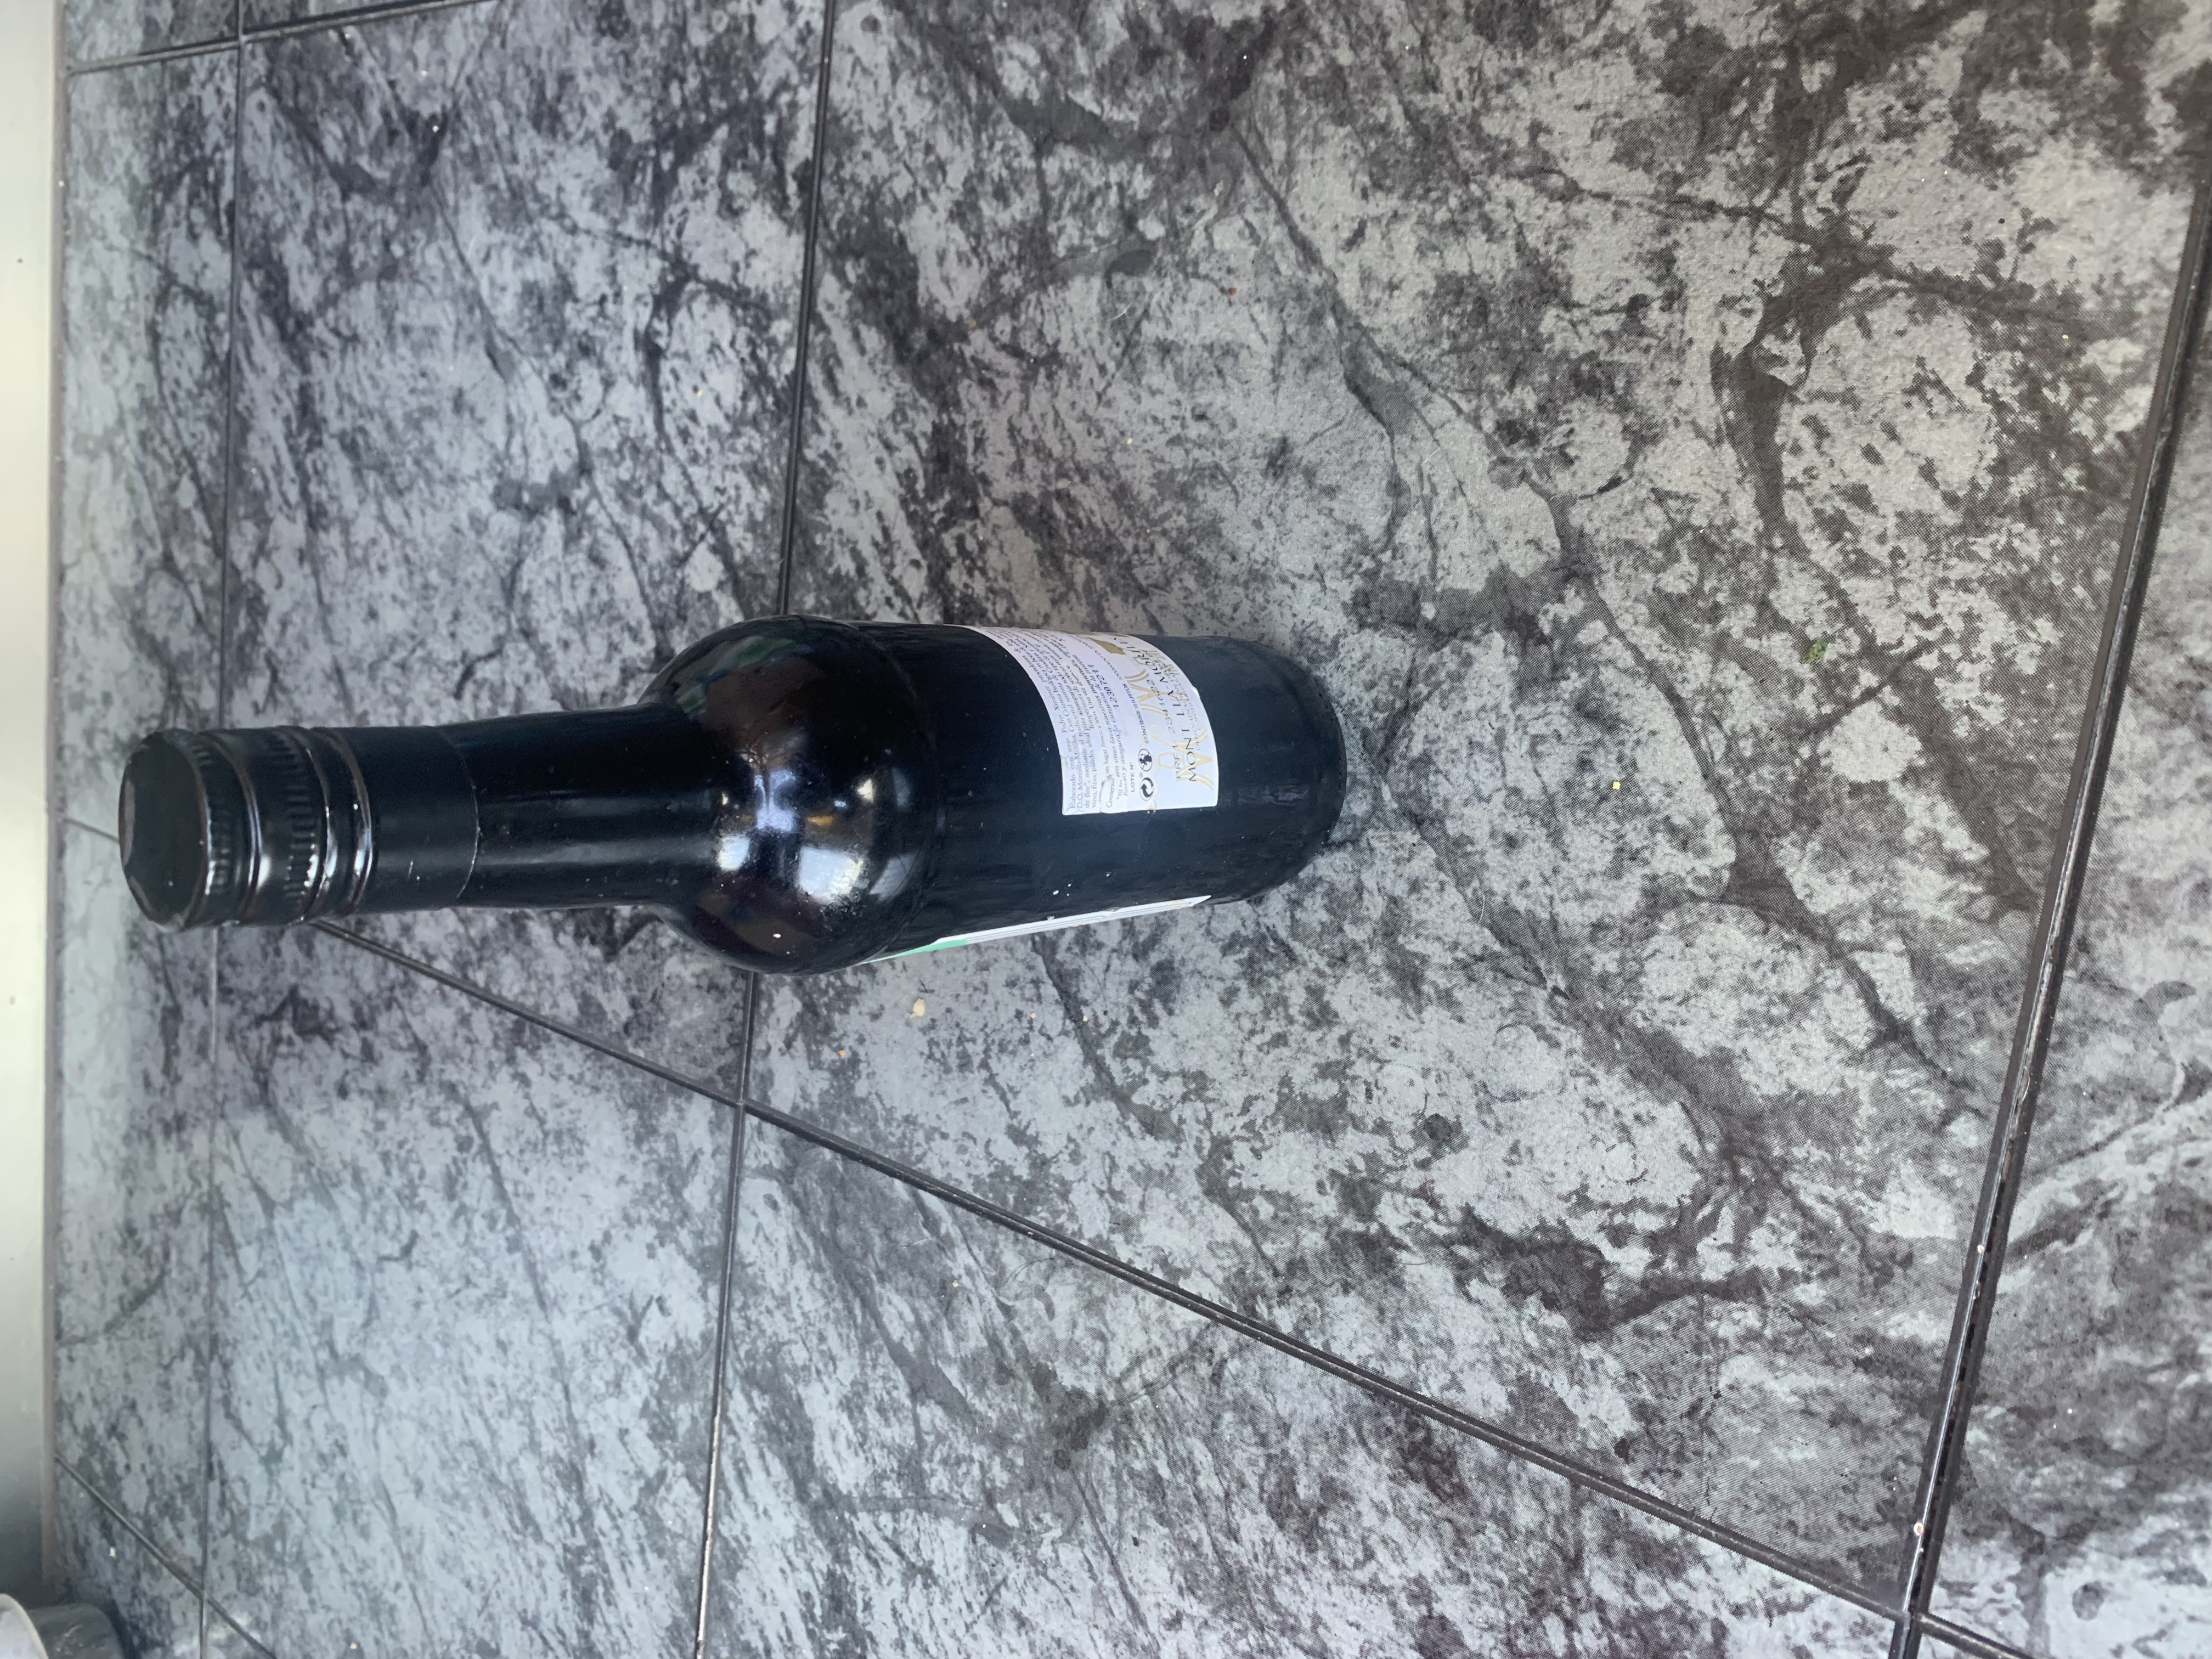
\includegraphics[width=0.12\textwidth]{img/green1.jpg}}{}
\stackunder[5pt]{
\includegraphics[width=0.12\textwidth]{img/green2.jpg}}{}
\stackunder[5pt]{\includegraphics[width=0.12\textwidth]{img/green.jpg}}{}
\stackunder[5pt]{\includegraphics[width=0.12\textwidth]{img/green3.jpg}}{}
\caption{Imatges d'exemple contenidor verd del dataset}
\end{figure}

\begin{figure} [!h]
\footnotesize
\stackunder[5pt]{\includegraphics[width=0.13\textwidth]{img/brown1.jpg}}{}
\stackunder[5pt]{\includegraphics[width=0.1\textwidth]{img/brown2.jpg}}{}
\stackunder[5pt]{\includegraphics[width=0.15\textwidth]{img/brown.jpg}}{}
\stackunder[5pt]{\includegraphics[width=0.1\textwidth]{img/brown3.jpg}}{}
\caption{Imatges d'exemple contenidor marró del dataset}
\end{figure}

 \subsubsection{Xarxa neural}
La xarxa neural és una part molt important del projecte, i el primer contacte amb la visió per computador del projecte. Aquesta és essencial per donar la intel·ligència al robot per poder classificar objectes.
\\

Per aconseguir-ho he utilitzat una xarxa neural convolucional (CNN) que forma part de la família DenseNet, aquesta xarxa es caracteritza pel seu disseny dens i connectivitat directa entre les capes. La xarxa utilitzada és una DenseNet-121, una xarxa preentrenada amb la qual es divideix en dues parts:

\begin{itemize}
  \item Pooling: És el nom que es dona a l'agrupació de diverses capes convolucionals.
  \item Unitats denses: Aquestes es componen de capes convolucionals en cascada, on cada capa rep connexions directes de totes les capes anteriors.
\end{itemize}

\begin{figure}[h]
 \centering
    \includegraphics[width=0.5\textwidth]{img/denseNet.png}
    \caption{Estructura d'una xarxa DenseNet}
\end{figure}
 \hfill \break

DenseNet-121 té un total de 121 capes, aquí s'inclouen les capes de convolució, agrupació i les capes completament connectades. A mesura que les dades flueixen per la xarxa es van extraient característiques a diferents nivells d'abstracció , el qual ens permet obtenir bastant detall i característiques a alt nivell de les imatges d'entrada.
\\

S'ha optat per aquest tipus de xarxa, pel fet que té un alt rendiment en les tasques de classificació d'imatges i no només en la classificació sinó que també ha donat molt bons resultats en detecció d'objectes, reconeixement d'objectes i en la segmentació semàntica.

\paragraph{Entrenament}

A l'hora d'entrenar la xarxa neural s'ha de tenir molts conceptes a tenir en compte, aquest poden ser opcionals com és el cas del preprocessament d'imatges..., i d'altres que són obligatoris, però són difícils de trobar com els hiperparàmetres \textit{batch}, \textit{epoch} i \textit{steps}.
\\

Per evitar un sobreentrenament de la xarxa, les imatges passen per un preprocessament on els realitza una augmentació de les dades, una rotació, un zoom, un redimensionament i un flip horitzontal. Amb això aconsegueixo una generalització i abstracció, pel fet que la xarxa rep una mateixa imatge de diferents formes i serà capaç de generalitzar millor i, per tant, classificarà millor una imatge que mai hagi vist.
\\

Per altra banda, també he hagut de modificar els pesos de les capes 34, ja que és una xarxa preentrenada i els pesos predefinits per defecte, no servien en aquest cas, la modificació dels pesos és automàtica mitjançant aquesta aprenent.
\\
 \hfill \break
(Consultí l’annex A.4 per veure el codi utilitzat a l'hora de crear la xarxa neural.)

 \hfill \break
\subsection{Orientació d'objecte}

L'orientació d'objectes és una eina en la visió per computador per determinar en quina direcció estova un objecte en una imatge o vídeos. Aquest tipus de codi s'enfoca a identificar i classifica l'orientació dels objectes detectats.
\\

Com he mencionat abans, la intenció de l'algorisme es detecta l'orientació de l'objecte, en aquest projecte n'és útil per saber en quina orientació el robot ha d'agafar el mateix, així doncs pot agafar la majoria dels objectes que se li presentin.
\\

A grans trets, l'algorisme fa un blur a la imatge recollida i a una imatge del fons (imatge de l'escena sense cap objecte), seguidament es fa una resta de les imatges per veure les diferències, la diferència serà l'objecte introduït a la cinta, per acabar és binaritza i es fa una erosió i dilatació, d'aquesta manera podem obtenir la silueta de l'objecte, un cop tenim aquesta imatge processada es busca el contorn i es calcula l'angle.
\\
 \hfill \break

(Consultí l’annex A.5 per veure el codi utilitzat a l'hora d'obtenir l'orientació d'un objecte.)

\subsection{Simulació}

Tal com es menciona en els objectius, un dels objectius finals és la creació d'una simulació en el programa Stäubli Robotic Suite 2022 (SRS). Aquest software ens permet treballar únicament amb els robots de l'empresa Stäubli, però d'una manera fàcil, amigable i el més real possible, ja que es poden simular tots els components del robot i entrades del controlador per fer una simulació el més pròxim a la realitat possible, també ens permet programar des de la posada en marxa del robot fins a l'aturada, optimització del rendiment, detecció i previsió de col·lisions, calibració, entre molts altres avantatges. Aquest simulador utilitza el mateix llenguatge que el robot real (VAL 3), d'aquesta manera es pot fer un port directe sense haver de transcriure el codi.
\\

L'escena creada conta de diversos objectes 3D, en la qual trobem el robot, el manipulador, un cub (simula un objecte), papereres de diferents colors i una taula. L'escena intenta que sigui el més fiable a la realitat possible, tenint en compte les dimensions, etc. No només intenta reflectir la realitat en l'escena, sinó que en la funcionalitat també, és a dir, aquesta simulació té les mateixes prestacions que el codi pel robot físic, com la paral·lelització dels codis, comunicació amb els altres elements del projecte, etc.

\begin{figure}[!h]
 \centering
    \includegraphics[width=0.5\textwidth]{img/simulacio.png}
    \caption{Escena del simulador Stäubli Robotic Suite}
\end{figure}
 \hfill \break
\\
\\
\\
\\
\\
\\
\subsection{Món físic}

Anomenaré nom físic al conjunt d'elements físic que es poden manipular físicament, és a dir, el món real. El món físic és un món complicat per a visió per computador, ja que si no tenim un entorn molt controlat, pot sorgir problemes a l'hora d'obtenir una imatge i s'hauria de realitzar un preprocessat a la imatge obtinguda, si això passa es perd bastant de temps en arreglar la imatge, pel fet que s'ha de buscar un preprocessat que funcioni amb la majoria d'objectes, per evitar això he intentat crear un entorn el més ideal possible. Per aconseguir aquest entorn ideal he dir a terme diversos canvis en l'escena física.
\\

El primer canvi es tracta de la posició d'on es capta la imatge de l'objecte, en aquest punt tenia diverses opcions, però he optat en implementar la més versàtil i estable de totes, aquesta tracta de crear una estructura independent, la qual es pugui acoblar al lateral de la cinta. Aquesta és una composició d'elements metàl·lics amb una impressió 3D al final. Els elements metàl·lics són uns tubs, dissenyats per acoblar i desacoblar estructures el més ràpid possible.
\\

L'estructura té forma de 'C', amb aquesta forma el robot pot entrar dintre de l'estructura a l'hora d'agafar l'objecte de la cinta. En el punt més alt de l'estructura, tenim una impressió 3D la qual em permet col·locar el telèfon mòbil, que aquest es qui s'encarrega de captar la imatge de l'objecte.

\begin{figure}[h]
 \centering
  \subfloat[Estructura creada]{
   \label{f:estructura}
    \includegraphics[width=0.2\textwidth]{img/estructura.jpg}}
  \subfloat[Plànol de l'estructura]{
   \label{f:pànol}
    \includegraphics[width=0.23\textwidth]{img/estructuraMides.jpg}}
 \caption{Estructura}
 \label{f:tx60}
\end{figure}

El segon canvi que he realitzat és amb la llum, a causa del fet que és una habitació molt il·luminada entrava molta claredat i molta llum, la claredat ens va bastant bé, així la imatge surt més nítida i es pot identificar millor l'objecte, en canvi, la llum no és tan bona idea que passi aquesta pot ocasionar reflexos i ombres, les quals poden ser perjudicials a l'hora de classificar l'objecte. Per solucionar aquest problema es va posar una tela blanca bastant porosa, així la llum entrant és una llum més tènue i es manté la claredat de la sala.
\\

Per acabar, vaig canviar d'eina en el robot, pel fet que una vàlvula de succió, és l'eina que hi havia abans, no seria capaç d'agafar la majoria d'objectes, només pel fer que la vàlvula agafa objectes relativament plans, en canvi, una ampolla de plàstic no la podria agafar, ja que és un cilindre i quedarien forats buits per on sortiria l'aire, així que vaig canvia d'eina, aquesta és una pinça que es compon de dues estructures, la primera és un gripper\cite{Gripper} que es va demanar a l'empresa Stäubli i el segon és una impressió 3D per tindre una major distància i millor adherència.

\begin{figure}[!h]
 \centering
  \subfloat[Plànols gripper]{
   \label{f:Plànols_gripper}
    \includegraphics[width=0.265\textwidth]{img/gripper.png}}
  \subfloat[Gripper amb el disseny 3D]{
   \label{f:gripper3D}
    \includegraphics[width=0.3\textwidth]{img/grippe3D.JPG}}
 \caption{Pinça}
 \label{f:gripper}
\end{figure}

 \hfill \break
\\

(Consultí l’annex A.7 per veure les mides del gripper i el plànol del la impresió 3D.)

\subsection{Connexió entre components}

Una part important del projecte és la connexió entre els dispositius, aquestes connexions són important per enviar dades entre ells i fer diferents accions depenen d'aquestes, en aquest projecte he utilitzat 2 tipus de connexions, com he comentat en l'apartat 4, aquestes són, els sockets i IvCAM.
\\

La primera és la connexió socket, aquest tipus de connexions es fan servir a l'hora d'enviar dades entre dos dispositius, ja que són connexions bidireccionals, amb una estructura client-servidor i en cas de fer servir els sockets/TCP, com en aquest projecte, tens una garantia que la dada enviada és la correcta i que el destinatari ha rebut el missatge. Aquest tipus de connexió està implementada en dos llocs del projecte, aquest són:
\\
\\
\begin{itemize}
	\item \textbf{PLC- Controlador}: EL PLC envia una dada, dient si hi ha un objecte o no a la cinta, la dada enviada és un caràcter en ASCII, concretament una D (valor 100 en la taula ascii), indicant que hi ha un objecte i una C (valor 99 en la taula ascii), indicant el contrari. El controlador no envia res al PLC.

	\item \textbf{Controlador - Ordinador}: El controlador emet un senyal, per dir que està en funcionament, un cop està la connexió establerta, els dos components s'esperen fins que hi hagui un objecte a la cinta, un cop sindica que hi ha un objecte (la controladora ha rebut un 100, mitjançant la connexió anterior), aquest dos intercanviaran dades per indicar a quin contenidor va l'objecte. El valor que indica el contenidor és un valor ascii (48,49,50 o 51), representant (groc, blau, verd o marró respectivament).
\end{itemize}

El segon tipus de connexió és una connexió IvCam, la qual ens permet intercanviar un gran cúmul de dades entre una càmera i un dispositiu mitjançant la tecnologia sense fils. Aquesta connexió s'utilitza només quan s'ha de realitzar la fotografia, és a dir, només la podem veure en la connexió de la càmera amb l'ordinador. Per dur a terme aquesta connexió s'ha fet servir el programa IvCAM d'esesoft, per fer que funcioni el programa només s'ha d'instal·lar en els dos dispositius, els dos dispositius han d'estar connectats a la mateixa xarxa, i obrir el programa en els dos dispositius per portar a cap la connexió.

 \begin{figure}[!h]
 \centering
    \includegraphics[width=0.5\textwidth]{img/connexions.png}
    \caption{Diagrama de connexions}
\end{figure}

\section{Tests}
En aquest apartat es e¡mensionen tots els testos que s'ha arribat a fer en aquest projecte.

\subsection{Xarxa neural}

En la xarxa neural he fet diversos tipus de proves, aquestes proves no consisteixen en funcions de testeig, ja que en una xarxa neural no té gaire sentit posar un testing del codi, però sí del resultat que dona, per tant, el testeig realitzat és sobre els resultats que retorna la xarxa, aquest s'han realitzat en diferents espais de temps que ha durat el projecte. Els testos es poden dividir en tres grans grups.

\begin{itemize}
 	\item El primer és el menys rellevant, ja que és un test amb imatges del propi dataset, ja sigui de l'apartat de test, validació o entrenament. Realment, d'aquests testos no es poden treure gaires conclusions, pel fet que la xarxa neural ja ha vist dos d'aquest grup per aprendre.

	\item La segona prova amb la xarxa neural va ser amb imatges externes al dataset, però aquestes imatges van ser tractades per només veure l'objecte que m'interessa, el fons aplicat és un color uniforme, més o menys del mateix color de la cinta. Aquests testos són més interessants per extreure conclusions i comprovar el real funcionament de la xarxa.
\begin{figure}[!h]
 \centering
  \subfloat[Verd]{
   \label{f:Verd}
    \includegraphics[width=0.23\textwidth]{img/TestGreen.png}}
  \subfloat[Groc]{
   \label{f:groc}
    \includegraphics[width=0.25\textwidth]{img/TestYellow.png}}
\\
\subfloat[Blau]{
   \label{f:blau}
    \includegraphics[width=0.23\textwidth]{img/TestBlue.png}}
 \subfloat[Orgànic]{
   \label{f:Orgànic}
    \includegraphics[width=0.3\textwidth]{img/TestOrganic.png}}
 \caption{Test objectes que no estàn en el dataset amb fons uniforme}
 \label{f:tx60}
\end{figure}

	\item La tercera i última prova és amb objectes sense un fons uniforme, aquestes proves es van fer per veure la reacció de la xarxa en passar-li una imatge amb un fons bastant diferent entre si, i comprova que reconeix de la mateixa manera l'objecte a classificar.

\begin{figure} [h]
\footnotesize
\centering
\stackunder[1pt]{\includegraphics[width=0.23\textwidth]{img/test2.png}}{}
\stackunder[1pt]{\includegraphics[width=0.24\textwidth]{img/test3.png}}{}
\end{figure}

\begin{figure} [h]
\footnotesize
\centering
\stackunder[1pt]{\includegraphics[width=0.29\textwidth]{img/test4.png}}{}
\caption{Test objectes que no estàn en el dataset amb fons}
\end{figure}
\end{itemize}

\subsection{Orientació d'objectes}

Per testejar l'orientació d'objectes, he seguit el mateix procediment que en l'apartat anterior, és a dir, he fet la comprovació per veure el funcionament amb imatges de prova, aquestes imatges són extretes directament de com és l'escena final, per tant, es pot veure l'objecte sobre la cinta.

 \begin{figure}[!h]
 \centering
    \includegraphics[width=0.4\textwidth]{img/axes.png}
    \caption{Test Orientació}
\end{figure}

\section{Resultats}
\subsection{Xarxa neural}

El resultat de la xarxa neuronal s'ha avaluat utilitzant una matriu de confusió, una eina fonamental per analitzar el rendiment del model de classificació. La matriu de confusió proporciona una visió detallada de les prediccions del model en cada classe objectiu. S'ha observat, que la classificació és bastant correcte, tenint en compte els falsos positius i falsos negatius, això indica que la xarax pot classificar imatges sense problemes.
\\

En particular, s'ha de destacar la classe "organic" i la classe "green" aquestes són les classes que tenen millors resultats a l'hora de classificar, ja que es confon bastant poc.
\\

No obstant això, s'ha identificat una major dificultat en la classificació de la classe "yellow". Aquesta classe en particular requereix més atenció i possiblement es beneficiaria d'un enfocament d'entrenament addicional o la inclusió de més dades representatives, pel fet que la classe la confon amb la classe "green", dedueixo, que és perquè tots dos són objectes transparents, de colors i poden tenir formes bastats semblants.
\\

En general, la matriu de confusió reflecteix un rendiment bastant sòlid del model en la tasca de classificació d'imatges.

 \begin{figure}[!h]
 \centering
    \includegraphics[width=0.5\textwidth]{img/ConfusionMatrix.png}
    \caption{Confusion Matrix}
\end{figure}
 \hfill \break

\subsection{Simulació i món fisic}

El resultat del projecte en aquest àmbit és similar en els dos casos, ja que són més o menys complementàries i es pot dir que compleix la funció esperada seguint un flux, aquest és el següent: s'inicien el programa de la xarxa neural i el robot, un cop els dos encesos el robot es mourà fins a arribar a un punt, on esperarà que el PLC mira si hi ha un objecte i envia el resultat, de si ha detectat un objecte o no. A continuació farà dues tasques al mateix temps, la primera és trametre a l'ordinador (on escroba tot el codi amb la xarxa neural) un senyal indicant que pot fer una fotografia, aquests li trametrà el senyal al telèfon mòbil i es realitzarà la fotografia i la guardarà, aquesta serà processada en la xarxa neural i per últim remetrà el resultat, la segona tasca que es realitza en paral·lel és el moviment del robot aproximant-se a la cinta per agafar l'objecte, aquest l'agafarà i espera en un punt a sobre de les papereres, esperant a rebre el resultat de la xarxa neural, un cop el rebi, deixarà el robot a la paperera corresponent i tornarà a començar.
\\

El flux abans comentat el podem veure a la següent figura, figura 18.
 
 \begin{figure}[!h]
 \centering
    \includegraphics[width=0.5\textwidth]{img/flux.png}
    \caption{Flux de tot el projecte}
\end{figure}
\hfill \break
\\
\\
\\
\\
\\
\\
\\
\\
\\
\\
\\
(Consultí l’annex A.6 per veure el codi implementat.)

\section{Conclusions i millores}

Gràcies a aquest projecte s'ha pogut descobrir un gran potencial en la Visió per computador, aplicant-la a un món que cada cop agafa més força com és la indústria 4.0. La xarxa neuronal DenseNet-121 és un clar exemple que es pot aplicar xarxes neuronals a molts àmbits, ja que no són gens rígides/enfocades a un únic treball, sinó que és una eina molt flexible i amb un potencial enorme, si volem un exemple, aquest projecte n'és un, en el qual s'ha aplicat una xarxa neural, que pot classificar en 4 classes, però afegint imatges al dataset sobre noves classes la mateixa xarxa podria ser una bona opció, només faria falta que tornes a aprendre.
\\

També he pogut experimentar la importància d'una metodologia àgil i tenir un pla B, segurament hi ha projectes que no és tan important, però en aquest en concret ha sigut bastant crucial el fet de poder anar avançant mentre alguna altra tasca no estava completa, un exemple d'això és el gripper el qual va triga bastant tard a l'hora de rebre'l, no obstant es podia continuar avançant per un altre camí i les proves que ha calgut fer, s'han fet amb una altra eina com un succionador, que encara no sigui el mateix em permetia poder avançant i fer les proves necessàries.
\\

Com a millora personal en aquest projecte el que faria és l'obtenció de l'objecte sense que la cinta hagi d'aturar-se, el qual estava previst d'implementar, però no s'ha pogut realitzar pel fet que la targeta que va acoblada al CS8C i pugui llegir un encoder, no ha arribat. Un altre millora que es podria fer és afegir diversos sensors, com sensors de pes..., splits per posar els objectes tan centrats com sigui possible a la cinta, etc.
\\

Per acabar, voldria mencionar que això té un propòsit com a eina per ajudar al reciclatge, ja que vivim en una època plena de residus, i els recursos no són il·limitat, per tant, amb aquest projecte s'intenta millorar la sostenibilitat mediambiental i ajudar a les plantes de residus a poder reciclar.

\section*{Agraïments}

Vull expressar el meu més sincer agraïment al meu tutor/a, Carlos García Calvo,  per la seva valuosa orientació i suport al llarg d'aquest projecte de reciclatge. La seva experiència, coneixements i dedicació han estat fonamentals per al meu creixement i èxit en aquesta iniciativa. Estic profundament agraït per la seva guia constant, la seva disposició per resoldre els meus dubtes i la seva motivació. La seva influència ha deixat una empremta en el desenvolupament projecte, i estic sincerament agraït per l'oportunitat de treballar sota la seva tutela.


%\begin{thebibliography}{11}
%\bibitem{latex}
%http://en.wikibooks.org/wiki/LaTeX

%\bibitem{2}
%Referència 2

%\bibitem{3}
%Etc.


%\end{thebibliography}
\bibliographystyle{IEEEtran} % We choose the "plain" reference style
\bibliography{IEEEabrv, refs} % Entries are in the refs.bib file

\clearpage 
\appendix

\section*{Apèndix}

\setcounter{section}{1}

\subsection{Objectius}


\begin{table}[h]
\begin{tabular}{ | m{1.5cm} | m{6cm} | }
\hline
\rowcolor[HTML]{C0C0C0}
\multicolumn{1}{|c|}{\textbf{CODI}} 	& \multicolumn{1}{c|}{\textbf{DESCRIPCIÓ}} 									\\ \hline
\multicolumn{1}{|c|}{{[}O1{]}} 	& Obtenir informació important sobre el robot TX-60 i simulador.							\\ \hline
\multicolumn{1}{|c|}{{[}O2{]}} 	& Realitzar la identificació d’objectes. 											\\ \hline
\multicolumn{1}{|c|}{{[}O3{]}} 	& Buscar informació sobre la programació del robot i el simulador. 							\\ \hline
\multicolumn{1}{|c|}{{[}O4{]}} 	& Crear una simulació realista del projecte.										\\ \hline
\multicolumn{1}{|c|}{{[}O5{]}} 	& Realitzar que la simulació funcioni en el món real i faci el circuit (agafar de la cinta, traslladar-ho al lloc).	\\ \hline
\multicolumn{1}{|c|}{{[}O6{]}} 	& Manipulació d’un objecte estàtic, en simulació com en espai real.							\\ \hline
\multicolumn{1}{|c|}{{[}O7{]}} 	& Realització d’agafar un objecte no estàtic.										\\ \hline
\multicolumn{1}{|c|}{{[}O8{]}} 	& Comunicar un ordinador amb el robot, per poder enviar-li accions a realitzar.					\\ \hline
\multicolumn{1}{|c|}{{[}O9{]}} 	& Utilització d’una pinça pneumàtica											\\ \hline
\multicolumn{1}{|c|}{{[}O10{]}} 	& Creació de les extensions de la pinça per poder agafar objectes.							\\ \hline
\end{tabular}
\end{table}

\subsection{Especificacións}
\subsubsection{Staubli Tx60 caracteristiques}

\begin{table}[h]
\begin{tabular}{ |l|l| }
\hline
\textbf{Marca} 		& Stäubli 						\\ \hline
\textbf{Model} 		& TX60						\\ \hline
\textbf{Tipus} 		& Braç robotic (braç antropomòrfic) 		\\ \hline
\textbf{Axes (joins)} 	& 6 							\\ \hline
\textbf{Carrega}		&3,5kg						\\ \hline
\textbf{Eixos} 		& 600 mm						\\ \hline
\textbf{Repetibilitat} 	& 0.02 mm						\\ \hline
\textbf{Pes} 		& 51 kg						\\ \hline
\end{tabular}
\end{table}

\subsection{Primeres pases}
\subsubsection{Codi ordinador python}

\begin{lstlisting}[language=Python]
import socket

sock = socket.socket(socket.AF_INET, socket.SOCK_STREAM)
server_address = ('XXX.XXX.XXX.XXX', XXXX)
sock.connect(server_address)
message = ''

try:
    message = b'0'
    print('sending {!r}'.format(message))
    sock.sendall(message)
    amount_received = 0
    amount_expected = len(message)
    while amount_received < amount_expected:
        data  = sock.recv(16)
        amount_received += len(data)
        print('received {!r}'.format(data))

finally:
    sock.close()

\end{lstlisting}

\subsubsection{Codi stäubli}

\begin{lstlisting}[language=Python]
cls()
movej(JHome,tTool, mNomSpeed)
waitEndMove()
movej(JApproach1,tTool, mNomSpeed)
waitEndMove()
do
    nTest = sioGet(sSioOrdenador, l_nNumero)
    sioGet(sSioPLC, l_nNumPLC)
    delay(5)
    put("Test connect to computer :")
    putln(nTest)
    put(" L_nNumero :")
    putln(l_nNumero)
    put(" L_nNumPLC :")
    putln(l_nNumPLC)
 
  until l_nNumero == 13
\end{lstlisting}

\subsection{Xarxa Neural}
\subsubsection{main.py}
\begin{lstlisting}[language=Python]
import tensorflow as tf
from tensorflow.keras.applications.densenet import preprocess_input
import classModels

imageSize = (224, 224)
batch_size = 32
names_class = ['blue', 'green', 'organic', 'yellow']

train_path = './dataset/train'
test_path = './dataset/test'
validation_path = './dataset/valid'

train_batches = tf.keras.preprocessing.image.ImageDataGenerator(
        rotation_range=5,
        rescale=1./255,
        horizontal_flip=True,
        zoom_range=0.2,
).flow_from_directory(
        directory=train_path,
        target_size=imageSize,
        classes=names_class,
        batch_size=batch_size,
        class_mode='categorical'
)
valid_batches = tf.keras.preprocessing.image.ImageDataGenerator(
        preprocessing_function=preprocess_input
).flow_from_directory(
        directory=validation_path,
        target_size=imageSize,
        classes=names_class,
        batch_size=batch_size,
        class_mode='categorical'
)

test_batches = tf.keras.preprocessing.image.ImageDataGenerator(
        preprocessing_function=preprocess_input,
).flow_from_directory(
        directory=test_path,
        target_size=imageSize,
        classes=names_class,
        batch_size=batch_size,
        shuffle=False,
        class_mode='categorical'
)
test_batches_nopre = tf.keras.preprocessing.image.ImageDataGenerator(
        dtype='uint8'
).flow_from_directory(
        directory=test_path,
        target_size=imageSize,
        classes=names_class,
        batch_size=batch_size,
        shuffle=False,
        class_mode='categorical'
)
epoch = 20
steps = int(train_batches.samples / 35)
val_steps = int(valid_batches.samples / 35)

secondModel = classModels.modelsDenseNet121(epoch, steps, val_steps, train_batches, valid_batches, test_batches, test_batches_nopre, True)

secondModel.baseModelDenseNet121()
secondModel.layerFalse(34)
secondModel.compileModel()
secondModel.fit()
\end{lstlisting}

\subsubsection{classModel.py}

\begin{lstlisting}[language=Python]
import tensorflow as tf
from tensorflow import keras

from keras import regularizers
from tensorflow.keras.layers import Flatten, Dense, Dropout, Input
from tensorflow.keras import Model
from tensorflow.keras.models import load_model
from tensorflow.keras.optimizers import SGD
from sklearn.metrics import confusion_matrix
from tensorflow.keras.applications.densenet import preprocess_input
from keras.callbacks import EarlyStopping, ReduceLROnPlateau

import numpy as np

class modelsDenseNet121:
    def __init__(self, epoch, steps, val_steps, train_batches, valid_batches, test, test_prepro, optimization=False):
        self.base_model = ''
        self.model = ''
        self.base_predic = ''
        self.predic = ''
        self.confusion = ""
        self.historic = ''
        self.callbackList = ''
        self.model_prepro = ""
        self.epoch = epoch
        self.steps = steps
        self.val_steps = val_steps
        self.train_batches = train_batches
        self.valid_batches = valid_batches
        self.testData = test
        self.optimization = optimization
        self.test_nopre = test_prepro

    def __init__(self, nameModel):
        self.loadModel(nameModel)

    def baseModelDenseNet121(self):
        self.base_model = tf.keras.applications.DenseNet121(weights='imagenet', include_top=False, pooling='avg')

        x = self.base_model.output
        x = Flatten()(x)
        x = Dense(256, kernel_regularizer=regularizers.l1_l2(0.01), activity_regularizer=regularizers.l2(0.01), activation='relu')(x)
        x = Dropout(0.5)(x)
        self.base_predic = Dense(4, activation='softmax')(x)

        self.model = Model(inputs=self.base_model.input, outputs=self.base_predic)

    def compileModel(self):
        if self.optimization:
            self.model.compile(optimizer=SGD(learning_rate=0.01, momentum=0.9), loss='categorical_crossentropy',
                               metrics=['accuracy', 'mse'])
            stop = EarlyStopping(monitor='val_loss', patience=8, verbose=1, min_delta=1e-4)
            reduceLr = ReduceLROnPlateau(monitor='val_loss', factor=0.1, patience=2, verbose=1, min_delta=1e-6)
            self.callbackList = [stop, reduceLr]

        else:
            self.model.compile(optimizer='adam', loss='categorical_crossentropy', metrics=['accuracy', 'mse'])
            stop = EarlyStopping(monitor='val_loss', patience=8, verbose=1, min_delta=1e-4)
            reduceLr = ReduceLROnPlateau(monitor='val_loss', factor=0.1, patience=3, verbose=1, min_delta=1e-4)
            self.callbackList = [stop, reduceLr]

    def fit(self):
         self.historic=self.model.fit(
             self.train_batches,
             steps_per_epoch=self.steps,
             validation_steps=self.val_steps,
             validation_data=self.valid_batches,
             epochs=self.epoch,
             callbacks=self.callbackList,
             verbose=1
         )

    def layerFalse(self, num=0):
        if num == 0:
            for layer in self.base_model.layers:
                layer.trainable = False
        else:
            for layer in self.model.layers[:num]:
                layer.trainable = False
            for layer in self.model.layers[num:]:
                layer.trainable = True

    def evaluateModel(self, preproc):
        if preproc:
            self.model.evaluate(x=self.test_nopre, verbose=1, steps=self.val_steps)
        else:
            self.model.evaluate(x=self.testData, verbose=1, steps=self.val_steps)

    def predictions(self, preproc=False):
        if preproc:
            self.predic = self.model.predict(x=self.test_nopre, verbose=1, steps=self.val_steps)
        else:
            self.predic = self.model.predict(x=self.testData, verbose=1, steps=self.val_steps)

\end{lstlisting}
\clearpage 
\subsection{Orientació d'objectes}
\begin{lstlisting}[language=Python]
import numpy as np
import cv2
import matplotlib.pyplot as plt

image = cv2.imread("./img/3bfce634-ab0c-4223-84c7-c20df6f6b48d.png")
backgound = cv2.imread("./background.png")

imgResult = cv2.cvtColor(image, cv2.COLOR_BGR2RGB)

image_blur = cv2.GaussianBlur(image, (51, 51), cv2.BORDER_DEFAULT)
image_bw = cv2.cvtColor(image_blur, cv2.COLOR_BGR2GRAY)

backblur = cv2.GaussianBlur(backgound, (51, 51), cv2.BORDER_DEFAULT)
back_bw = cv2.cvtColor(backblur, cv2.COLOR_BGR2GRAY)

diff = cv2.absdiff(image_bw, back_bw)
ret, mascara = cv2.threshold(diff, 30, 255, cv2.THRESH_BINARY)

kernel_1 = np.ones((5, 5), np.uint8)
mascara = cv2.erode(mascara, kernel_1, iterations=5)
mascara = cv2.dilate(mascara, kernel_1, iterations=2)

kernel_2 = np.ones((7, 7), np.uint8)
mascara = cv2.dilate(mascara, kernel_2, iterations=20)
mascara = cv2.erode(mascara, kernel_2, iterations=10)

contours = cv2.findContours(mascara, cv2.RETR_EXTERNAL, cv2.CHAIN_APPROX_SIMPLE)[-2]

rotrect = cv2.minAreaRect(contours[0])

cv2.drawContours(imgResult, contours, 0,(255,0,0),2)

angle = rotrect[-1]
if angle < -45:
    angle = -(90 + angle)
else:
    angle = angle

return angle

\end{lstlisting}

\subsection{Codi final}
\subsubsection{Codi principal ordinador}
\begin{lstlisting}[language=Python]
import classModels
import orientationDetector
import cv2
import uuid
import socket

tcpsocket = socket.socket(socket.AF_INET, socket.SOCK_STREAM)
sock = socket.socket(socket.AF_INET, socket.SOCK_STREAM)
server_address = ('XXX.XXX.XXX.XXX', XXXX)
sock.connect(server_address)

data = sock.recv(16)
cap = cv2.VideoCapture(0)

names_class = ['blue', 'green', 'organic', 'yellow']
model = classModels.modelsDenseNet121("modelUse")

takeFoto = False
stopProgram = False

if data == b'I':
    while not(stopProgram):
        while not(takeFoto):
            data = sock.recv(16)
            if data == b'R':
                takeFoto = True
        leido, frame = cap.read()

        if leido:
            nameFoto = './img/' +str(uuid.uuid4()) + ".png"
            cv2.imwrite(nameFoto, frame)
            angle = orientationDetector.getOrientation(nameFoto)
	 sock.sendall(angle)

            resultClass = model.classifyImage(names_class, nameFoto)
            sock.sendall(resultClass)

        else:
            stopProgram = True
        takeFoto = False

cap.release()
sock.close()
\end{lstlisting}

\subsubsection{codi prncipal controladora}
\begin{lstlisting}[language=Python]
begin
  movej(JHome,tToolSuccion, mNomSpeed)
  waitEndMove()
  movej(JApproach1,tToolSuccion, mNomSpeed)
  waitEndMove()
  do
    movel(pTable,tToolSuccion, mNomSpeed)
    waitEndMove()
    sioGet(sPlc, nRecvPLC)
    if nRecvPLC == 100
      sioSet(sSocket, 82)
      movej(jAproachCinta, tToolSuccion, mNomSpeed)
      waitEndMove()
      movej(jGetCinta, tToolSuccion, mNomSpeed)
      waitEndMove()
      close(tToolSuccion)
      waitEndMove()
      movel(pApprBins, tToolSuccion, mNomSpeed)
      waitEndMove()
      nConnection = sioGet(sSocket, nRecvData)
    switch nRecvData
      case 48
        movel(pBinYellow, tToolSuccion, mNomSpeed)
        waitEndMove()
      break
      case 49
        movel(pBinBlue, tToolSuccion, mNomSpeed)
        waitEndMove()
      break
      case 50
        movel(pBinGreen, tToolSuccion, mNomSpeed)
        waitEndMove()
      break
      case 51
        movel(pBinBrown, tToolSuccion, mNomSpeed)
        waitEndMove()
      break
      default
        putln("Bin selected no correct")
      break
    endSwitch
      open(tToolSuccion)
      waitEndMove()
      nRecvPLC=0
      clearBuffer(sPlc)
    endIf
  until 1==2
end
\end{lstlisting}
 
\subsection{Pinça}
\subsubsection{Mides gripper}

\begin{table}[h]
\begin{tabular}{ |m {0.5 cm}|m {0.5 cm}|m {0.5 cm}|m {0.5 cm}|m {0.5 cm}|m {0.5 cm}|m {0.5 cm}|m {0.5 cm}|m {0.5 cm}|m {0.5 cm}|m {0.5 cm}|m {0.5 cm}|m {0.5 cm}| }
\hline
\multicolumn{1}{|c|}{\begin{tabular}[c]{@{}c@{}}A \\ {[}mm{]}\end{tabular}} &
\multicolumn{1}{c|}{\begin{tabular}[c]{@{}c@{}}A1 \\ {[}mm{]}\end{tabular}} &
\multicolumn{1}{c|}{\begin{tabular}[c]{@{}c@{}}B \\ {[}mm{]}\end{tabular}} &
\multicolumn{1}{c|}{\begin{tabular}[c]{@{}c@{}}C \\ {[}mm{]}\end{tabular}} &
\multicolumn{1}{c|}{\begin{tabular}[c]{@{}c@{}}C1 \\ {[}mm{]}\end{tabular}} &
\multicolumn{1}{c|}{\begin{tabular}[c]{@{}c@{}}C2 \\ {[}mm{]}\end{tabular}} &
\multicolumn{1}{c|}{\begin{tabular}[c]{@{}c@{}}D \\ {[}mm{]}\end{tabular}} &
\multicolumn{1}{c|}{\begin{tabular}[c]{@{}c@{}}D1 \\ {[}mm{]}\end{tabular}} &
\multicolumn{1}{c|}{\begin{tabular}[c]{@{}c@{}}E1 \\ {[}mm{]}\end{tabular}} &
\multicolumn{1}{c|}{\begin{tabular}[c]{@{}c@{}}E2 \\ {[}mm{]}\end{tabular}} &
\multicolumn{1}{c|}{\begin{tabular}[c]{@{}c@{}}E3 \\ {[}mm{]}\end{tabular}} &
\multicolumn{1}{c|}{\begin{tabular}[c]{@{}c@{}}F1 \\ {[}mm{]}\end{tabular}} & 
\multicolumn{1}{c|}{\begin{tabular}[c]{@{}c@{}}F2 \\ {[}mm{]}\end{tabular}} \\ \hline

\multicolumn{1}{|c|}{44} & 
\multicolumn{1}{c|}{67} & 
\multicolumn{1}{c|}{34} & 
\multicolumn{1}{c|}{142} & 
\multicolumn{1}{c|}{138} & 
\multicolumn{1}{c|}{98} & 
\multicolumn{1}{c|}{46} & 
\multicolumn{1}{c|}{45.5} & 
\multicolumn{1}{c|}{7} & 
\multicolumn{1}{c|}{9} & 
\multicolumn{1}{c|}{9} & 
\multicolumn{1}{c|}{19.5} & 
\multicolumn{1}{c|}{19.5} \\ \hline
\end{tabular}
\end{table}

\begin{table}[h]
\begin{tabular}{ |m {0.5 cm}|m {0.5 cm}|m {0.5 cm}|m {0.5 cm}|m {0.5 cm}|m {0.5 cm}|m {0.5 cm}|m {0.5 cm}|m {0.5 cm}|m {0.5 cm}|m {0.5 cm}|m {0.5 cm}|m {0.5 cm}| }
\hline
\multicolumn{1}{|c|}{\begin{tabular}[c]{@{}c@{}}F3 \\ {[}mm{]}\end{tabular}} &
\multicolumn{1}{c|}{\begin{tabular}[c]{@{}c@{}}G \\ {[}mm{]}\end{tabular}} &
\multicolumn{1}{c|}{\begin{tabular}[c]{@{}c@{}}H \\ {[}mm{]}\end{tabular}} &
\multicolumn{1}{c|}{\begin{tabular}[c]{@{}c@{}}H1 \\ {[}mm{]}\end{tabular}} &
\multicolumn{1}{c|}{\begin{tabular}[c]{@{}c@{}}H2 \\ {[}mm{]}\end{tabular}} &
\multicolumn{1}{c|}{\begin{tabular}[c]{@{}c@{}}K \\ {[}mm{]}\end{tabular}} &
\multicolumn{1}{c|}{\begin{tabular}[c]{@{}c@{}}L \\ {[}mm{]}\end{tabular}} &
\multicolumn{1}{c|}{\begin{tabular}[c]{@{}c@{}}L1 \\ {[}mm{]}\end{tabular}} &
\multicolumn{1}{c|}{\begin{tabular}[c]{@{}c@{}}R \\ {[}mm{]}\end{tabular}} &
\multicolumn{1}{c|}{\begin{tabular}[c]{@{}c@{}}S \\ {[}mm{]}\end{tabular}} &
\multicolumn{1}{c|}{\begin{tabular}[c]{@{}c@{}}T \\ {[}mm{]}\end{tabular}} &
\multicolumn{1}{c|}{\begin{tabular}[c]{@{}c@{}}U \\ {[}mm{]}\end{tabular}} & 
\multicolumn{1}{c|}{\begin{tabular}[c]{@{}c@{}}V \\ {[}mm{]}\end{tabular}} \\ \hline

\multicolumn{1}{|c|}{20} & 
\multicolumn{1}{c|}{M5} & 
\multicolumn{1}{c|}{M4} & 
\multicolumn{1}{c|}{M4} & 
\multicolumn{1}{c|}{M4} & 
\multicolumn{1}{c|}{15} & 
\multicolumn{1}{c|}{10} & 
\multicolumn{1}{c|}{3} & 
\multicolumn{1}{c|}{4.5} & 
\multicolumn{1}{c|}{54} & 
\multicolumn{1}{c|}{52} & 
\multicolumn{1}{c|}{34} & 
\multicolumn{1}{c|}{42} \\ \hline
\end{tabular}
\end{table}

\subsubsection{Mides de l'impresió 3D}
 \begin{figure}[!h]
 \centering
    \includegraphics[width=0.3\textwidth]{img/planol3d.png}
    \caption{Mides (en milìmetres) de l'estructura 3D }
\end{figure}

\end{document}

